\documentclass[tikz,border=8pt]{standalone}
\usepackage[T1]{fontenc}
\usepackage{lmodern}
\usepackage{amsmath}
\usetikzlibrary{arrows.meta, positioning, fit}

\definecolor{boxbg}{HTML}{F8FAFC}
\definecolor{boxline}{HTML}{334155}
\definecolor{stagebg}{HTML}{EFF6FF}
\definecolor{stageborder}{HTML}{2563EB}
\definecolor{listbg}{HTML}{F8FAFC}
\definecolor{actorbg}{HTML}{EEF2FF}
\definecolor{criticbg}{HTML}{ECFDF5}
\definecolor{pointerbg}{HTML}{FFF7ED}
\definecolor{outbg}{HTML}{FEFCE8}

\tikzset{
  box/.style={
    draw=boxline,
    rounded corners=5pt,
    line width=0.8pt,
    fill=boxbg,
    align=left,
    inner sep=7pt,
    font=\sffamily\small
  },
  stage/.style={
    box,
    fill=stagebg,
    draw=stageborder,
    minimum height=16mm,
    align=center,
    font=\sffamily\bfseries\small
  },
  listbox/.style={
    box,
    fill=listbg,
    text width=56mm
  },
  widebox/.style={
    box,
    text width=96mm
  },
  actorbox/.style={
    box,
    fill=actorbg,
    text width=48mm
  },
  criticbox/.style={
    box,
    fill=criticbg,
    text width=42mm
  },
  pointerbox/.style={
    box,
    fill=pointerbg,
    text width=64mm
  },
  simplebox/.style={
    box,
    fill=boxbg,
    text width=46mm
  },
  outbox/.style={
    box,
    fill=outbg,
    align=center,
    minimum width=32mm
  },
  arrow/.style={
    -{Latex[length=2.5mm]},
    line width=0.8pt,
    draw=boxline
  },
  softarrow/.style={
    -{Latex[length=2.2mm]},
    line width=0.7pt,
    draw=boxline
  }
}

\begin{document}
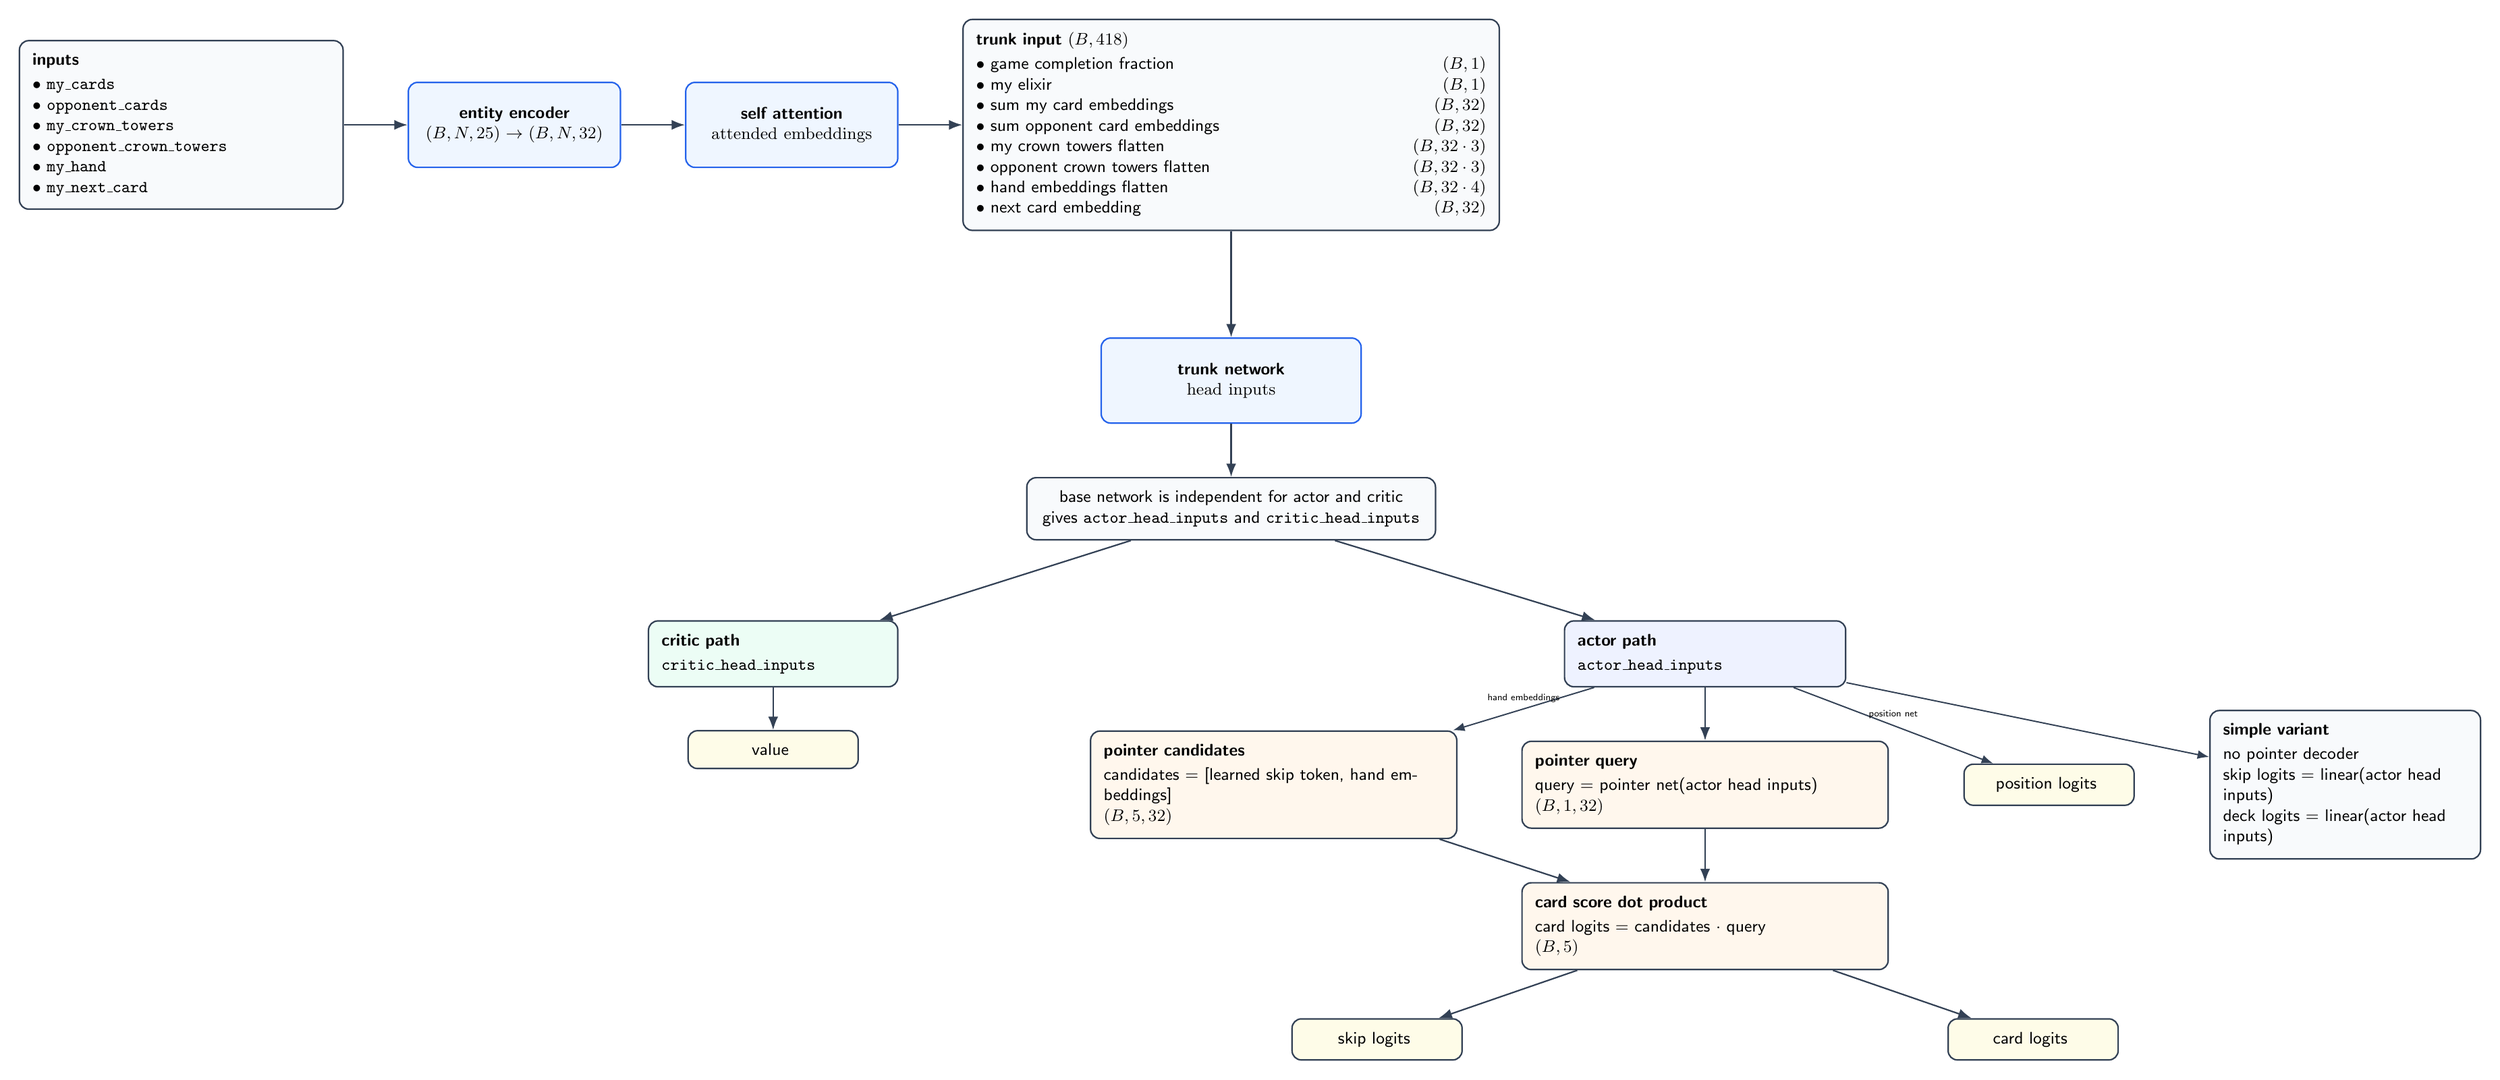
\begin{tikzpicture}[node distance=11mm and 12mm]

\node[listbox] (inputs) {
  \textbf{inputs}\\[2pt]
  $\bullet$ \texttt{my\_cards}\\
  $\bullet$ \texttt{opponent\_cards}\\
  $\bullet$ \texttt{my\_crown\_towers}\\
  $\bullet$ \texttt{opponent\_crown\_towers}\\
  $\bullet$ \texttt{my\_hand}\\
  $\bullet$ \texttt{my\_next\_card}
};

\node[stage, right=of inputs, text width=35mm] (encoder) {
  entity encoder\\
  \normalfont $(B,N,25)\to(B,N,32)$
};

\node[stage, right=of encoder, text width=35mm] (attention) {
  self attention\\
  \normalfont attended embeddings
};

\node[widebox, right=of attention] (trunkinput) {
  \textbf{trunk input} $(B,418)$\\[2pt]
  $\bullet$ game completion fraction \hfill $(B,1)$\\
  $\bullet$ my elixir \hfill $(B,1)$\\
  $\bullet$ sum my card embeddings \hfill $(B,32)$\\
  $\bullet$ sum opponent card embeddings \hfill $(B,32)$\\
  $\bullet$ my crown towers flatten \hfill $(B,32\cdot3)$\\
  $\bullet$ opponent crown towers flatten \hfill $(B,32\cdot3)$\\
  $\bullet$ hand embeddings flatten \hfill $(B,32\cdot4)$\\
  $\bullet$ next card embedding \hfill $(B,32)$
};

\node[stage, below=20mm of trunkinput, text width=44mm] (trunk) {
  trunk network\\
  \normalfont head inputs
};

\node[box, below=10mm of trunk, text width=72mm, align=center] (split) {
  base network is independent for actor and critic\\
  gives \texttt{actor\_head\_inputs} and \texttt{critic\_head\_inputs}
};

\node[criticbox, below left=15mm and 24mm of split] (critic) {
  \textbf{critic path}\\[2pt]
  \texttt{critic\_head\_inputs}
};

\node[outbox, below=8mm of critic] (value) {
  value
};

\node[actorbox, below right=15mm and 24mm of split] (actor) {
  \textbf{actor path}\\[2pt]
  \texttt{actor\_head\_inputs}
};

\node[pointerbox, below=10mm of actor] (query) {
  \textbf{pointer query}\\[2pt]
  query $=$ pointer net(actor head inputs)\\
  $(B,1,32)$
};

\node[pointerbox, left=12mm of query] (candidates) {
  \textbf{pointer candidates}\\[2pt]
  candidates $=$ [learned skip token, hand embeddings]\\
  $(B,5,32)$
};

\node[pointerbox, below=10mm of query] (dot) {
  \textbf{card score dot product}\\[2pt]
  card logits $=$ candidates $\cdot$ query\\
  $(B,5)$
};

\node[outbox, below left=9mm and 11mm of dot] (skip) {
  skip logits
};

\node[outbox, below right=9mm and 11mm of dot] (deck) {
  card logits
};

\node[outbox, right=14mm of query] (pos) {
  position logits
};

\node[simplebox, right=14mm of pos] (simple) {
  \textbf{simple variant}\\[2pt]
  no pointer decoder\\
  skip logits $=$ linear(actor head inputs)\\
  deck logits $=$ linear(actor head inputs)
};

\draw[arrow] (inputs) -- (encoder);
\draw[arrow] (encoder) -- (attention);
\draw[arrow] (attention) -- (trunkinput);
\draw[arrow] (trunkinput.south) -- (trunk.north);
\draw[arrow] (trunk) -- (split);
\draw[arrow] (split) -- (critic);
\draw[arrow] (critic) -- (value);
\draw[arrow] (split) -- (actor);
\draw[arrow] (actor) -- (query);
\draw[softarrow] (actor) -- node[above, font=\sffamily\tiny] {hand embeddings} (candidates);
\draw[arrow] (query) -- (dot);
\draw[arrow] (candidates) -- (dot);
\draw[arrow] (dot) -- (skip);
\draw[arrow] (dot) -- (deck);
\draw[softarrow] (actor) -- node[above, font=\sffamily\tiny] {position net} (pos);
\draw[softarrow] (actor) -- (simple);

\end{tikzpicture}
\end{document}
